\documentclass[12pt]{extarticle}
\usepackage[english,ukrainian]{babel}
\usepackage[utf8]{inputenc}
\usepackage{amsmath,amssymb}
\usepackage{parskip}
\usepackage{graphicx}
\usepackage{xcolor}
\usepackage{tcolorbox}
\tcbuselibrary{skins}
\usepackage[framemethod=tikz]{mdframed}
\usepackage{chngcntr}
\usepackage{enumitem}
\usepackage{hyperref}
\usepackage{float}
\usepackage{subfig}
\usepackage{chngcntr}
\usepackage{esint}

\usepackage[top=2.5cm, left=3cm, right=3cm, bottom=4.0cm]{geometry}
\usepackage[table]{xcolor}

\usepackage{algorithm}
\usepackage{algpseudocode}
\usepackage{listings}
\usepackage{xcolor}

\definecolor{codegreen}{rgb}{0,0.6,0}
\definecolor{codegray}{rgb}{0.5,0.5,0.5}
\definecolor{codepurple}{rgb}{0.58,0,0.82}
\definecolor{backcolour}{rgb}{0.95,0.95,0.92}

\lstdefinestyle{mystyle}{
    backgroundcolor=\color{backcolour},   
    commentstyle=\color{codegreen},
    keywordstyle=\color{magenta},
    numberstyle=\tiny\color{codegray},
    stringstyle=\color{codepurple},
    basicstyle=\ttfamily\footnotesize,
    breakatwhitespace=false,         
    breaklines=true,                 
    captionpos=b,                    
    keepspaces=true,                 
    numbers=left,                    
    numbersep=5pt,                  
    showspaces=false,                
    showstringspaces=false,
    showtabs=false,                  
    tabsize=2
}
\lstset{style=mystyle}

\usepackage{ragged2e}
\begin{document}

\begin{titlepage}
	\centering
	
\includegraphics[width=0.15\textwidth]{images/lab_1/logo.png}\par\vspace{0.3cm}
	{\textbf{Міністерство освіти і науки України}\par
 Харківський національний університет імені В.Н. Каразіна\par}
    \vspace{1cm}
	{\Large \textsc{Лабораторна робота \#1}\par
    \textbf{Інтерполяція функцій поліномами за формулами Лагранжа і Ньютона}\par}
	\vfill
 \begin{FlushRight}
	\textbf{Виконав:}\par Захаров Дмитро Олегович \par Група МП-31
\end{FlushRight}
	\vfill

% Bottom of the page
	{\large Харків -- 2023\par}
\end{titlepage}

\tableofcontents
\pagebreak

\section{Постановка задачі}

Побудувати інтерполяційний поліном Лагранжа і Ньютона (вперед та назад) $L_n(x)$, $N_n^+(x)$, $N_n^{-}(x)$ для функції $f(x)$, заданої в вузлах відрізку $[\alpha,\beta]$ значеннями $f(x_i),\, i \in \{0,\dots,n\}$:
\begin{enumerate}
    \item $x_k = \alpha+k\cdot h, \; h = \frac{\beta-\alpha}{n}, \; k \in \{0,\dots,n\}$
    \item $\hat{x}_k = \frac{1}{2}\left(\beta+\alpha -(\beta-\alpha)\cos \frac{2k+1}{2(n+1)}\pi\right), \; k \in \{0,\dots,n\}$
\end{enumerate}

На друк вивести результати у вигляді таблиць:
\[
x_i^* \; \; \; \; \; f(x_i^*) \; \; \; \; \; P_n(x_i^*) \; \; \; \; \; |f(x_i^*) - P_n(x_i^*)|
\]
де $x_i^*=x_i+\alpha h, \; i \in \{0,\dots,n-1\}, \alpha \in (0,1)$, $P_n$ кожен з трьох поліномів $L_n(x),N_n^+(x),N_n^{-}(x)$ для випадків $1$ та $2$.

\textbf{Варіант 5.}
\[
f(x) = e^{\frac{x}{10}}\sin x + x^3 + \cos x, \; \alpha=-2, \; \beta = 2
\]

\pagebreak
\section{Опис методів}

\subsection{Інтерполяційний поліном Лагранжа}

Нехай маємо вузли $\{x_j\}_{j=0}^n \subset [\alpha,\beta]$ та значення функції $f: [\alpha,\beta] \to \mathbb{R}$ в них $\{f_j\}_{j=0}^n := \{f(x_j)\}_{j=0}^n$. Інтерполяційний поліном Лагранжа має вигляд:
\[
L_n(x) = \sum_{i=0}^n f_i\ell_i(x), \; \ell_i(x) \triangleq \prod_{j \neq i}^n \frac{x-x_j}{x_i-x_j}
\]

\subsection{Інтерполяційний поліном Ньютона}

Нехай маємо вузли $\{x_j\}_{j=0}^n \subset [\alpha,\beta]$ та значення функції $f: [\alpha,\beta] \to \mathbb{R}$ в них $\{f_j\}_{j=0}^n := \{f(x_j)\}_{j=0}^n$. Тоді, інтерполяційні поліноми Ньютона вперед та назад ($N_n^+(x)$ та $N_n^{-}(x)$, відповідно) мають вид:
\[
N_n^+(x) = \varphi_0 + \sum_{k=1}^n \varphi_{[0:k]}\prod_{i=0}^{k-1} (x-x_i), \; N_n^{-}(x) = \varphi_n + \sum_{k=1}^n \varphi_{[n:n-k]} \prod_{i=0}^{k-1} (x-x_{n-i})
\]
де
\[
y_{[i:j]} \triangleq \frac{y_{[i+1:j]}-y_{[i:j-1]}}{x_j-x_i}
\]

Значення розділених різниць можна рахувати і рекурсивно, але значно легше використати наступну формулу:
\[
y_{[i:i+k]} = \sum_{j=0}^{k} \frac{y_{i+j}}{\prod_{l=0,l\neq j}^k (x_{i+j} - x_{i+l})}
\]

\pagebreak
\section{Текст програми}

Повний текст програми можна знайти за \href{https://github.com/ZamDimon/University-Homeworks/tree/main/Term%205/Numerical%20Analysis/lab_1}{цим посиланням} ($\leftarrow$ напис клікабельний) на \textit{Github} сторінку.

\subsection{Генерація вузлів}

Для початку, створимо файл \texttt{generators.py}, завантажимо залежності та створимо свій тип для інтервалу:

\begin{lstlisting}[language=Python, caption=Завантаження залежностей]
from math import cos, pi
from typing import Tuple, TypeAlias, List
from abc import ABC, abstractmethod

Interval: TypeAlias = Tuple[float, float]
\end{lstlisting}

Зробимо генерацію вузлів через абстрактний клас, котрий буде вміти створюватись та генерувати набір $x$ координат вузлів через функцію \texttt{generate\_nodes}. Також, тут же задамо функцію \texttt{generate\_test\_points}, котра буде видавати набір $x$ координат точок, на котрих ми будемо оцінювати інтерполяцію (як сказано в умові, використовуючи формулу $x_i^* = x_i+\alpha h$ де $x_i$ це координата вузла).

\begin{lstlisting}[language=Python, caption=Задання абстрактного класу]
class IDataPointsGenerator(ABC):
    """Interface for generating data points"""
    
    def __init__(self, interval: Interval, number: int) -> None:
        """
        Function initializing the generator

        ### Args:
        - interval (`Interval`): Interval on which the data points will be generated
        - number (`int`): Number of data points to generate
        """
        
        assert number > 0, "Number of data points must be greater than 0"
        assert interval[0] < interval[1], "Lower bound must be less than upper bound"
        
        self._lower, self._upper = interval
        self._number = number
    
    @abstractmethod
    def generate_nodes(self) -> List[float]:
        """
        Function generating data points

        ### Returns:
            `List[float]`: List of generated x coordinates
        """
        pass
    
    @abstractmethod
    def generate_test_points(self, alpha: float = 0.1) -> List[float]:
        """
        Function generating test points for evaluating the polynomial
        ### Args:
        - alpha (`float`): We will evaluate the polynomial at points x_i + alpha*h

        Returns:
        - List[float]: List of x coordinates
        """
        
        nodes = self.generate_nodes()
        h = (self._upper - self._lower) / self._number
        return [node + alpha*h for node in nodes]
\end{lstlisting}

Далі, наводимо конкретні реалізації цього інтерфейсу.

\subsubsection{Лінійно розбитий проміжок}
\begin{lstlisting}[language=Python, caption=Генерація лінійно розкинутих точок]
class LinearDataPointsGenerator(IDataPointsGenerator):
    """Class for generating linearly spaced data points"""
    
    def __init__(self, interval: Interval, number: int) -> None:
        super().__init__(interval, number)
    
    def generate_nodes(self) -> List[float]:
        fn = lambda i: self._lower + i * (self._upper - self._lower) / (self._number)
        return [fn(i) for i in range(self._number + 1)]
    
    def generate_test_points(self, alpha: float = 0.1) -> List[float]:
        return super().generate_test_points(alpha)
\end{lstlisting}

\subsubsection{Проміжок розбитий по гармонічному закону}
\begin{lstlisting}[language=Python, caption=Генерація точок по закону з косинусом]
class CosineDataPointsGenerator(IDataPointsGenerator):
    """Class for generating cosine spaced data points"""
    
    def __init__(self, interval: Interval, number: int) -> None:
        super().__init__(interval, number)
        
    def generate_nodes(self) -> List[float]:
        fn = lambda i: 0.5*(self._lower+self._upper-(self._upper-self._lower)*cos((2*i+1)*pi/(2*(self._number+1))))
        return [fn(i) for i in range(self._number + 1)]

    def generate_test_points(self, alpha: float = 0.1) -> List[float]:
        return super().generate_test_points(alpha)
\end{lstlisting}

\subsubsection{Перевірка генерації}
Перевіримо роботу програми, поклавши $n:=4$ для нашого конкретного інтервалу $[-2,2]$. В коді, це виглядає так:

\begin{lstlisting}[language=Python, caption=Використання генераторів]
linear_generator = LinearDataPointsGenerator((-2.0, 2.0), 4)
cosine_generator = CosineDataPointsGenerator((-2.0, 2.0), 4)

print(f"Linear generator nodes: {linear_generator.generate_nodes()}")
print(f"Cosine generator nodes: {cosine_generator.generate_nodes()}")
\end{lstlisting}

Якщо запустити, отримаємо наступний результат:

\begin{lstlisting}[language=bash, caption=Результат запуску генераторів]
Linear generator nodes: [-2.0, -1.0, 0.0, 1.0, 2.0]
Cosine generator nodes: [-1.902113032590307, -1.1755705045849463, -1.2246467991473532e-16, 1.175570504584946, 1.902113032590307]
\end{lstlisting}

Перевіримо аналітично. У випадку лінійного розбиття, маємо:
\[
x_k = -2 + k \cdot \frac{2+2}{4} = -2 + k
\]

Дійсно, якщо підставляти $k \in \{0,\dots,4\}$, отримаємо точки $\{-2,-1,0,1,2\}$.

У випадку розбиття по косинусу:
\[
\hat{x}_k = \frac{1}{2}\left(2-2-(2+2)\cos \frac{2k+1}{10}\pi\right) = -2 \cos \frac{(2k+1)\pi}{10}
\]

Тому, наприклад, $\hat{x}_0 = -2\cos \frac{\pi}{10} \approx -1.902$. Аналогічно можна перевірити схожість для інших $k$. Отже, ми дійсно отримали схожі результати.

\subsection{Поліноми}

Створимо файл \texttt{polynomials.py} та завантажимо залежності:

\begin{lstlisting}[language=Python, caption=Завантаження залежностей]
from math import prod
from abc import ABC, abstractmethod
from typing import List, Tuple, TypeAlias

Point: TypeAlias = Tuple[float, float]
\end{lstlisting}

Знову створимо абстракцію для поліномів. Кожен поліном має мати конструктор, а також функцію \texttt{evaluate}, котра рахує значення полінома в заданій точці:

\begin{lstlisting}[language=Python, caption=Інтерфейс для поліномів]
class IPolynomial(ABC):
    """Interface any polymial should implement"""
    
    def __init__(self, points: List[Point]) -> None:
        """ 
        Initializes the polynomial
        ### Args:
        - points (`List[Point]`): List of points to interpolate on
        """
        assert len(points) > 1, "At least two points are required"
        self._points = points
    
    @abstractmethod
    def evaluate(self, x: float) -> float:
        """
        Evaluates the polynomial at x
        ### Args:
        - x (`float`): Point to evaluate the polynomial at
        ### Returns:
            `float`: Value of the polynomial at x
        """
        pass
\end{lstlisting}

Далі, наводимо конкретні реалізації для кожного з поліномів.

\subsubsection{Поліном Лагранжа}

\begin{lstlisting}[language=Python, caption=Реалізація полінома Лагранжа]
class LagrangePolynomial(IPolynomial):
    """Polynomial implementing Lagrange interpolation"""
    
    def __init__(self, points: List[Point]) -> None:
        super().__init__(points)
        
    def _lagrange_coefficient(self, i: int, x: float) -> float:
        """ Calculates the i-th Lagrange coefficient at x

        ### Args:
        - i (`int`): Number of the Lagrange coefficient to calculate
        - x (`float`): Point to calculate the Lagrange coefficient at

        ### Returns:
            float: Value of the i-th Lagrange coefficient at x
        """
        # Finding the i-th point's x coordinate
        x_i, _ = self._points[i]
        # Forming an array of product terms
        terms = [(x-x_j) / (x_i-x_j) for (j, (x_j,_)) in enumerate(self._points) if i!=j]
        # Finding their product
        return prod(terms)
        
    def evaluate(self, x: float) -> float:
        # Finding the y coordinate of each point and multiplying it by the corresponding Lagrange coefficient
        terms = [self._lagrange_coefficient(i, x) * y for (i, (_, y)) in enumerate(self._points)]
        # Summing the terms
        return sum(terms)
\end{lstlisting}

\subsubsection{Поліном Ньютона назад}

Тут, при інціалізації (функція \texttt{\_\_init\_\_}), ми спочатку рахуємо і зберігаємо набір роздільних різниць за допомогою внутрішньої функції \texttt{\_differential\_difference(self, i: int, j: int) -> float}, а далі при обрахунку значення (функція \texttt{evaluate}) використовуємо збереженні значення

\begin{lstlisting}[language=Python, caption=Реалізація полінома Ньютона назад]
class NewtonBackwardsPolynomial(IPolynomial):
    """Polynomial implementing Newton's lower interpolation"""
    
    def __init__(self, points: List[Point]) -> None:
        # Calculating all differential differences beforehand
        super().__init__(points)
        n = len(points)
        self._differences = [self._differential_difference(n-1, i) for i in reversed(range(n))]
        
    def _differential_difference(self, i: int, j: int) -> float:
        """ Finds the differential difference y[i:j] at given x

        ### Args:
        - x (`float`): Point to find the differential difference at
        - i (`int`): From which index to start
        - j (`int`): At which index to stop

        ### Returns:
            `float`: Value of a differential difference at x
        """
        assert i >= 0, "i must be positive"
        assert j <= len(self._points), "j must be less than the number of points"

        # It is easier to deal with indices i,...,i-k
        k = i - j
        sum_terms: List[float] = [] # Defining a list of terms to sum
        for j in range(k+1):
            # Finding the denominator product terms
            denominator_terms = [self._points[i-j][0] - self._points[i-l][0] for l in range(k+1) if l!=j]
            # Dividing the numerator (self._points[i+j][1]) by the product of denominator terms
            sum_terms.append(self._points[i-j][1] / prod(denominator_terms))
        
        return sum(sum_terms)
    
    def evaluate(self, x: float) -> float:
        # Defining a list of terms to sum
        n = len(self._points)
        sum_terms: List[float] = []
        for i in reversed(range(n)):
            product_terms = [x - X for (X, _) in self._points[i+1:n]]
            # Finding the differential difference y[0:i+1] at x
            sum_terms.append(self._differences[n-1-i] * prod(product_terms))
        
        return sum(sum_terms)
\end{lstlisting}

\subsubsection{Поліном Ньютона вперед}

Реалізація ідейно така сама, як і в попередній секції.

\begin{lstlisting}[language=Python, caption=Реалізація полінома Ньютона вперед]
class NewtonForwardPolynomial(IPolynomial):
    """Polynomial implementing Newton's upper interpolation"""
    
    def __init__(self, points: List[Point]) -> None:
        # Calculating all differential differences beforehand
        super().__init__(points)
        self._differences = [self._differential_difference(0, i) for i in range(len(points))]
        
    def _differential_difference(self, i: int, j: int) -> float:
        """ Finds the differential difference y[i:j] at given x

        ### Args:
        - x (`float`): Point to find the differential difference at
        - i (`int`): From which index to start
        - j (`int`): At which index to stop

        ### Returns:
            `float`: Value of a differential difference at x
        """
        assert i >= 0, "i must be greater than 0"
        assert j <= len(self._points), "j must not exceed the number of points"
        
        # It is easier to deal with indices i,...,i+k
        k = j - i
        
        sum_terms: List[float] = [] # Defining a list of terms to sum
        for j in range(k+1):
            # Finding the denominator product terms
            denominator_terms = [self._points[i+j][0] - self._points[i+l][0] for l in range(k+1) if l!=j]
            # Dividing the numerator (self._points[i+j][1]) by the product of denominator terms
            sum_terms.append(self._points[i+j][1] / prod(denominator_terms))
        
        return sum(sum_terms)
    
    def evaluate(self, x: float) -> float:
        # Defining a list of terms to sum
        sum_terms: List[float] = []
        for i in range(len(self._points)):
            product_terms = [x - x_j for (x_j, _) in self._points[:i]]
            # Finding the differential difference y[0:i+1] at x
            sum_terms.append(self._differences[i] * prod(product_terms))
        
        return sum(sum_terms)
\end{lstlisting}

\subsection{Програма для оцінки}

Тепер напишемо програму, котра оцінює поліноми і видає потрібні нам таблиці. 

Використаємо пакет \texttt{rich} для красивого виведення таблиць у консоль :)

Далі алгоритм простий: створюємо масив (або, аналогічно, словник) з генераторів та поліномів, а потім попарно проходимось і генеруємо $6$ таблиць. Скоріше за все, логіку з оцінювання по конкретним \texttt{IPolynomial} та \texttt{IDataPointsGenerator} можна було виділити окремо (власне, для цього і існують інтефрейси та абстрактні класи). Проте, не будемо і далі ускладнювати структуру програми і просто запишемо все в одній функції:

\begin{lstlisting}[language=Python, caption=Реалізація побудови таблиць з результатами]
# Math imports
from math import exp, sin, cos

# Internal imports
from generators import IDataPointsGenerator, LinearDataPointsGenerator, CosineDataPointsGenerator
from polynomials import LagrangePolynomial, NewtonForwardPolynomial, NewtonBackwardsPolynomial

# Rich logging
from rich.console import Console
from rich.table import Table

if __name__ == "__main__":
    # Defining the task parameters
    interval = (-2.0, 2.0)
    segments_number = 20
    alpha = 0.3
    fn = lambda x: exp(x / 10.0) * sin(x) + x**3 + cos(x)
    
    # Defining the generator and defining a set of points
    generators: dict[str, IDataPointsGenerator] = {
        "linear generation": LinearDataPointsGenerator(interval, segments_number),
        "cosine generation": CosineDataPointsGenerator(interval, segments_number)
    }
    
    # For rich logging
    console = Console()
    
    for generator_name, generator in generators.items():
        # Defining the points on which to interpolate the polynomial
        node_x = generator.generate_nodes()
        node_points = [(x, fn(x)) for x in node_x]
        
        # Defining the polynomials
        polynomials = {
            "Lagrange Polynomial": LagrangePolynomial(node_points),
            "Newton Forward Polynomial": NewtonForwardPolynomial(node_points),
            "Newton Backwards Polynomial": NewtonBackwardsPolynomial(node_points)
        }
        
        # Defining the test points
        test_x = generator.generate_test_points(alpha=alpha)
        test_points = [(x, fn(x)) for x in test_x]
        
        for polynomial_name, polynomial in polynomials.items():
            table = Table(title=f"{polynomial_name} evaluation using {generator_name}")
            table.add_column("x", justify="center", style="cyan", no_wrap=True)
            table.add_column("f(x)", justify="center", style="magenta")
            table.add_column("P(x)", justify="center", style="green")
            table.add_column("|f(x)-P(x)|", justify="center", style="blue")
        
            for test_point in test_points:
                x_label = "{:.18f}".format(test_point[0])
                f_x_label = "{:.18f}".format(test_point[1])
                p_x_label = "{:.18f}".format(polynomial.evaluate(test_point[0]))
                difference_label = "{:.18f}".format(abs(test_point[1] - polynomial.evaluate(test_point[0])))
                
                table.add_row(x_label, f_x_label, p_x_label, difference_label)

            console.print(table)
\end{lstlisting}

\pagebreak

\section{Результати}

Для експериментів ми взяли $n=20$ та $\alpha=0.3$. Якщо ви хочете спробувати вибрати інші параметри, то можете запустити програму, що прикріплена у додатку :)

\subsection{Лінійно розбитий проміжок}
\begin{figure}[H]
    \centering
    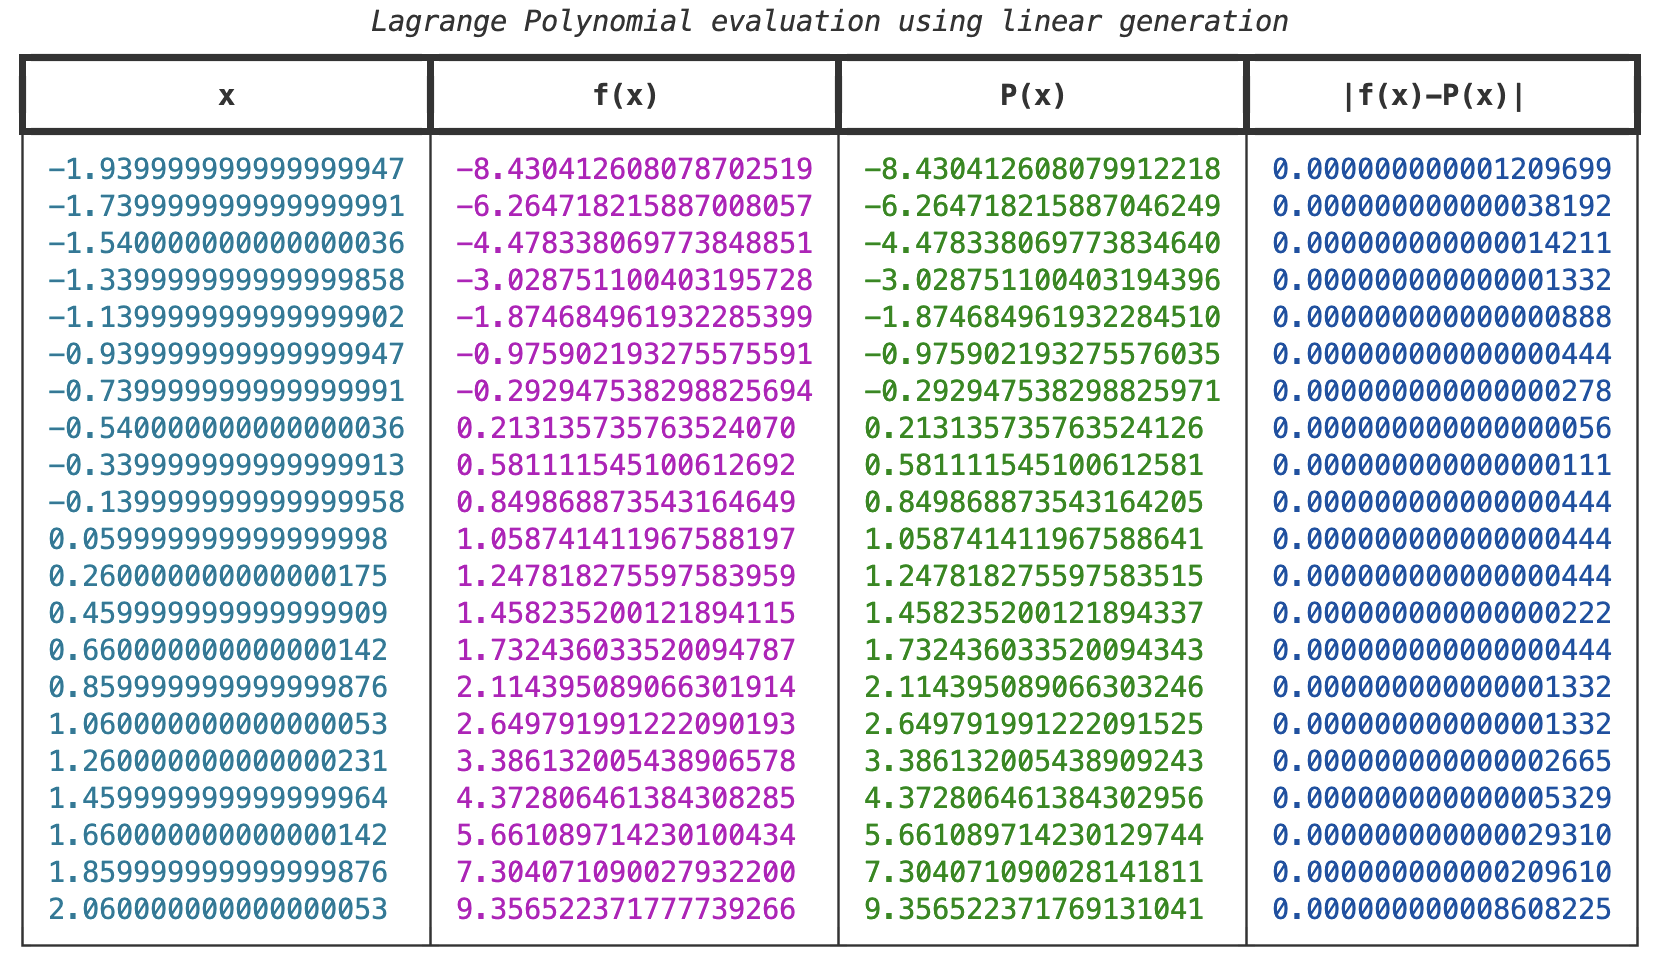
\includegraphics[width=\textwidth]{images/lab_1/lagrange_linear.png}
    \caption{Результат для полінома Лагранжа для лінійного розбиття}
    \label{fig:6}
\end{figure}
\vspace{5px}

\begin{figure}[H]
    \centering
    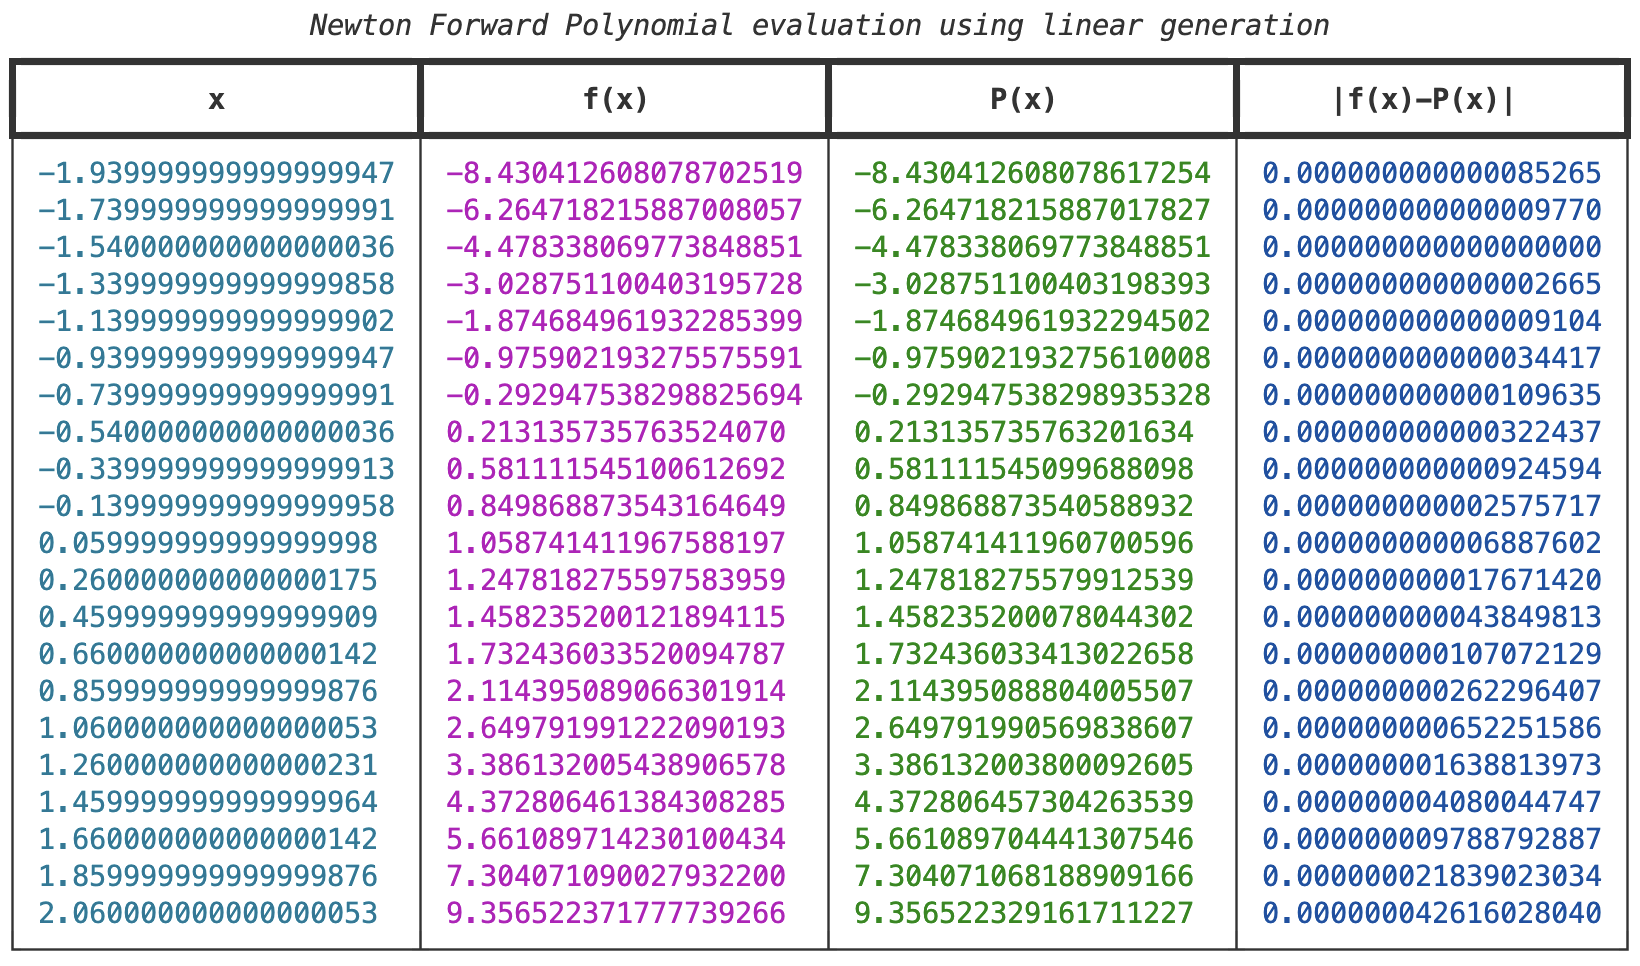
\includegraphics[width=\textwidth]{images/lab_1/newton_forw_linear.png}
    \caption{Результат для полінома Ньютона вперед для лінійного розбиття}
    \label{fig:6}
\end{figure}
\vspace{5px}

\begin{figure}[H]
    \centering
    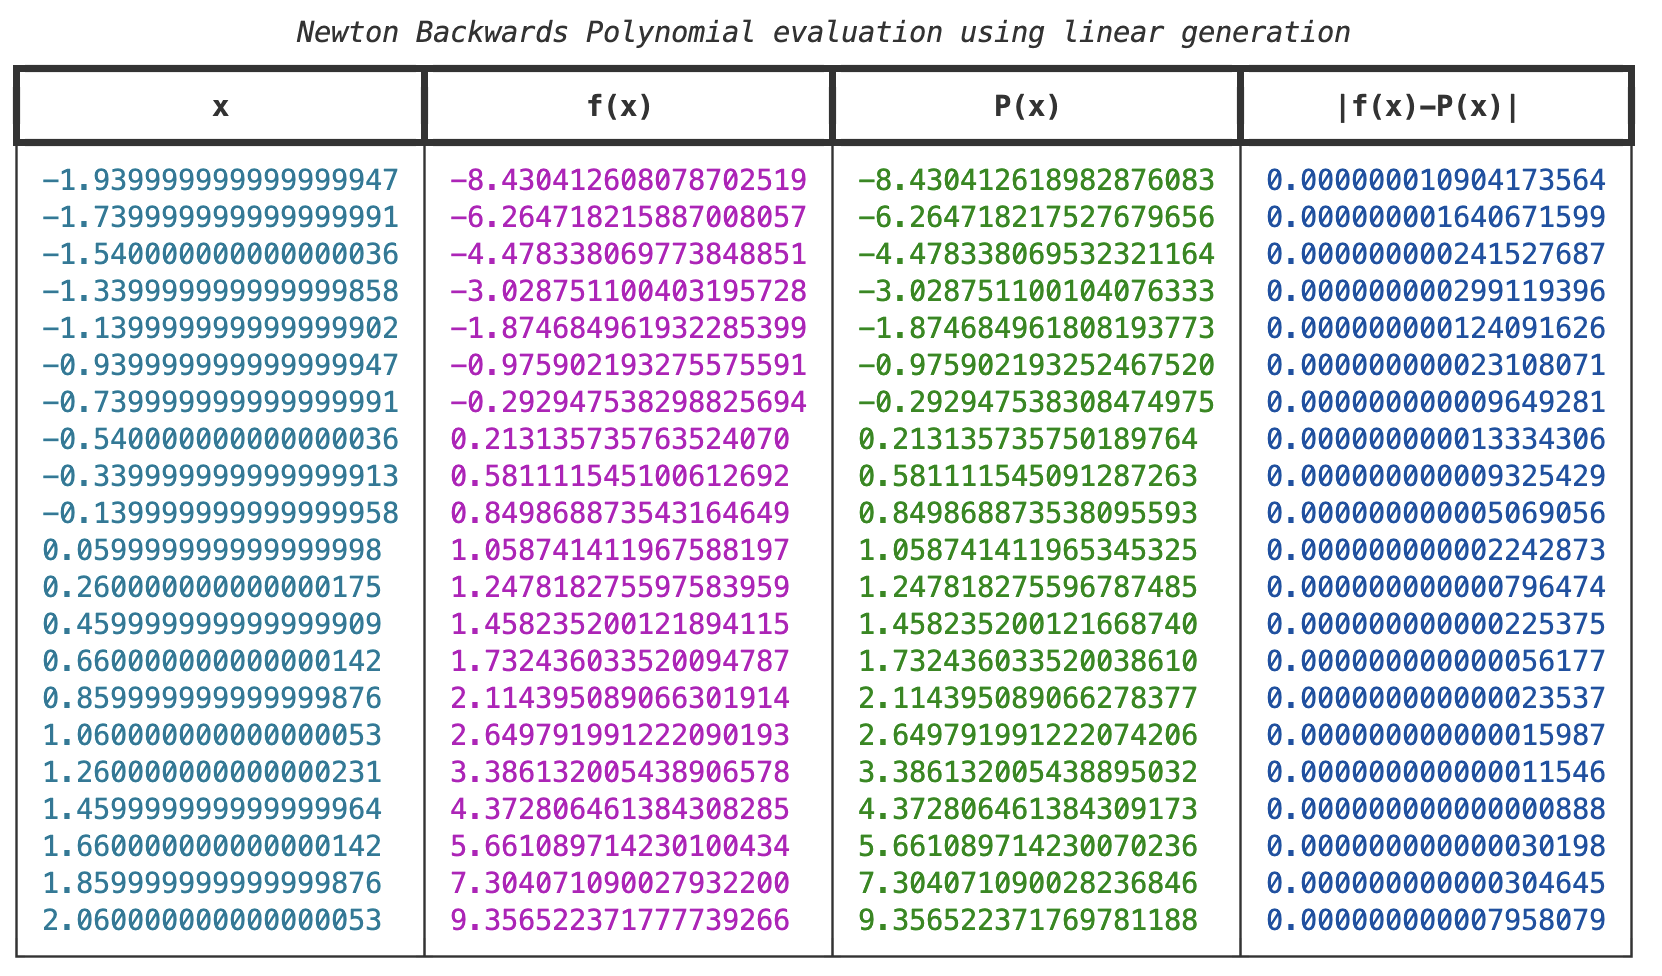
\includegraphics[width=\textwidth]{images/lab_1/newton_back_linear.png}
    \caption{Результат для полінома Ньютона назад для лінійного розбиття}
    \label{fig:6}
\end{figure}
\vspace{5px}

\subsection{Проміжок розбитий по гармонічному закону}

\begin{figure}[H]
    \centering
    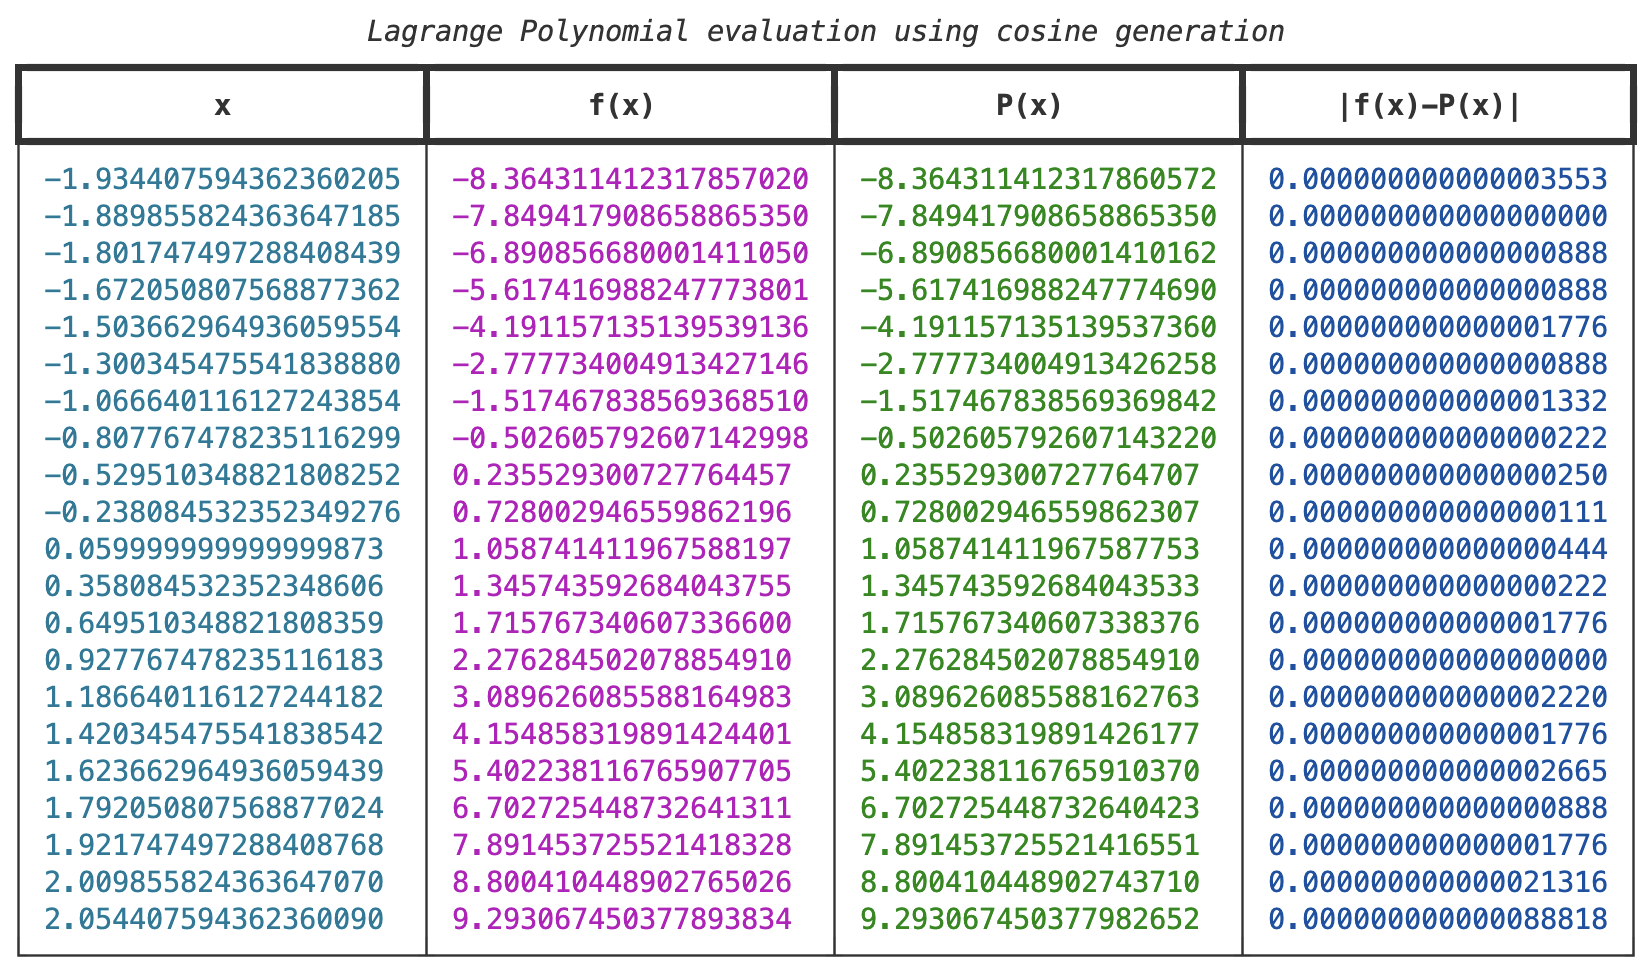
\includegraphics[width=\textwidth]{images/lab_1/lagrange_cosine.png}
    \caption{Результат для полінома Лагранжа для розбиття по косинусу}
    \label{fig:6}
\end{figure}
\vspace{5px}

\begin{figure}[H]
    \centering
    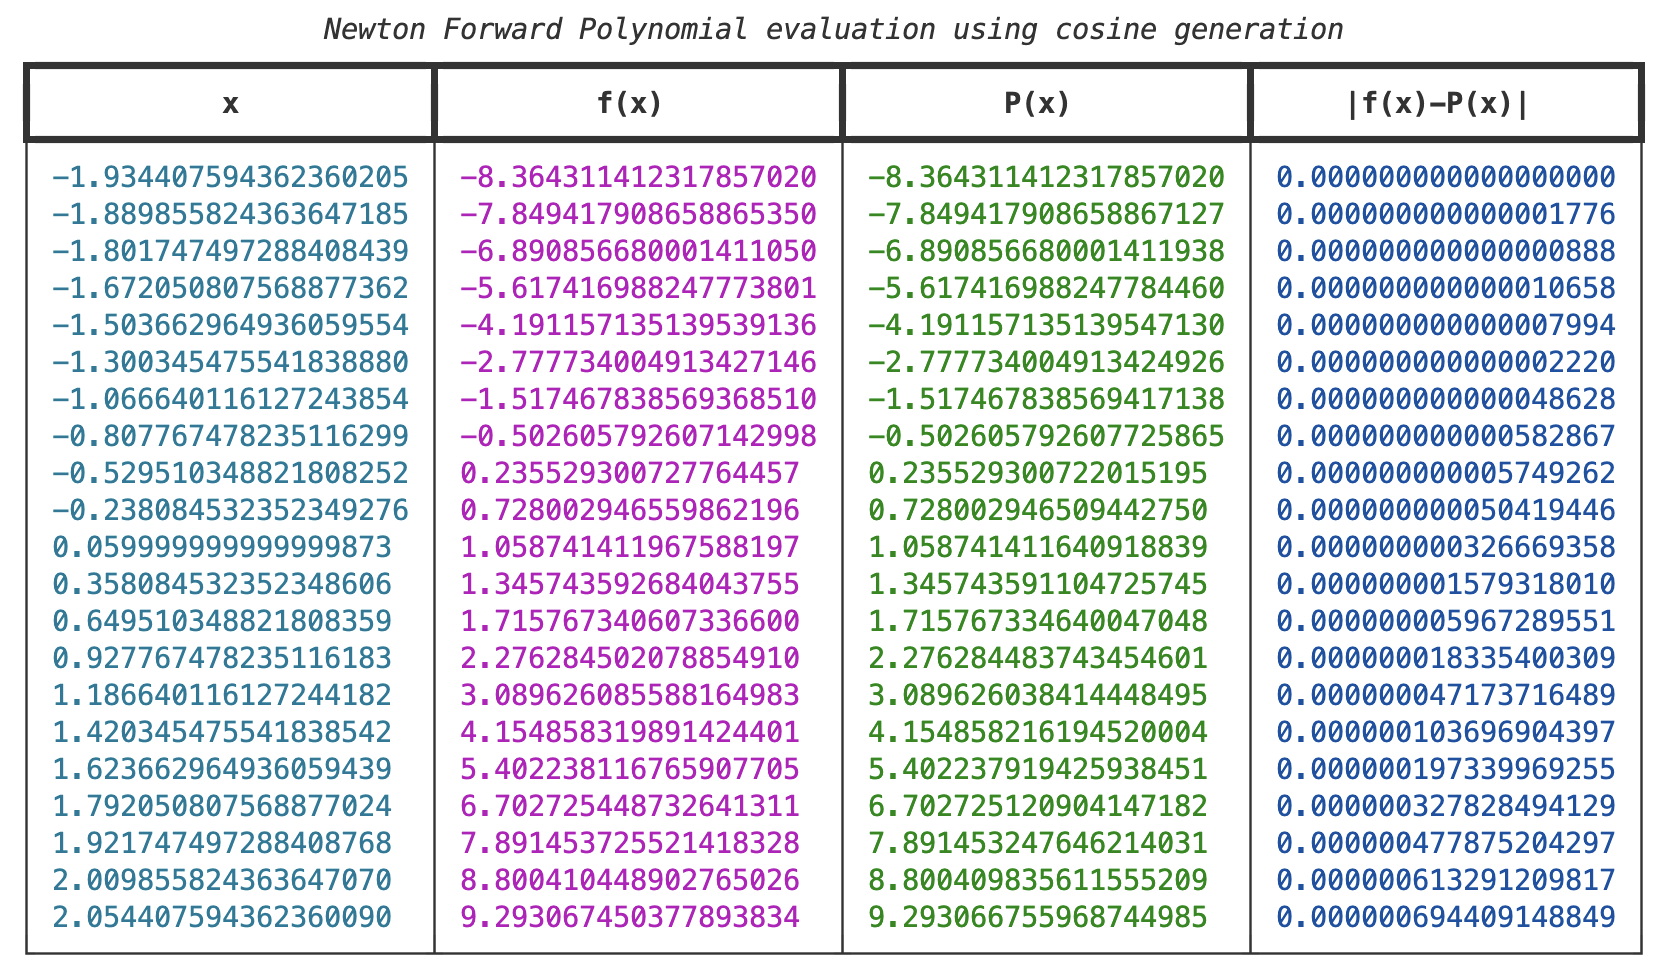
\includegraphics[width=\textwidth]{images/lab_1/newton_forw_cosine.png}
    \caption{Результат для полінома Ньютона вперед для розбиття по косинусу}
    \label{fig:6}
\end{figure}
\vspace{5px}

\begin{figure}[H]
    \centering
    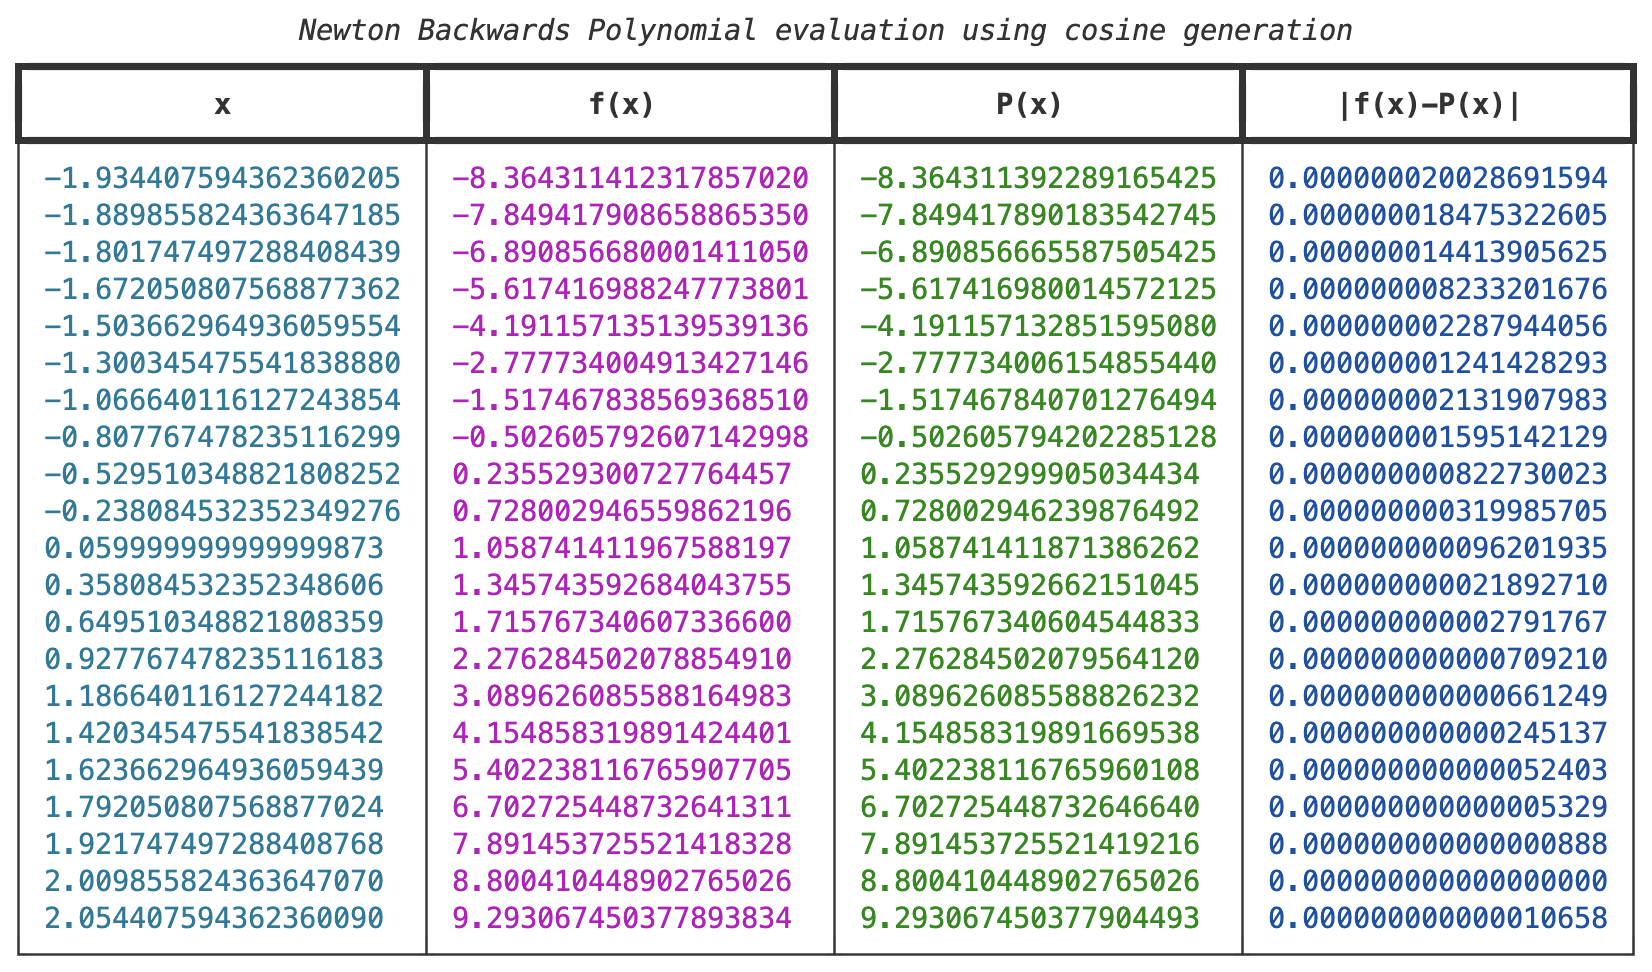
\includegraphics[width=\textwidth]{images/lab_1/newton_back_cosine.png}
    \caption{Результат для полінома Ньютона назад для розбиття по косинусу}
    \label{fig:6}
\end{figure}
\vspace{5px}

\section{Висновки}

В цій лабораторній роботі ми:
\begin{itemize}
\item навчилися будувати інтерполяційні поліноми Лагранжа, Ньютона вперед та Ньютона назад;
\item писати комп'ютерну програму (на прикладі мови \texttt{Python}), що будує вищезгадані поліноми;
\item оцінювати написану програму та діставати дані з експериментів.
\end{itemize}

Тепер більш детально про аналіз результатів. Як бачимо, в усіх випадках модуль різниці $|f(x^*)-P(x^*)|$ -- дуже мала величина, що говорить про точність інтерполяції на заданому проміжку (оскільки ми брали набір точок $x^*_i$, що відносно близький до вузлів $x_i$).

Порівняти 3 поліноми по точності доволі складно, оскільки в усіх випадках різниця дуже маленька (часто порядком нижче за $10^{-8}$): навіть якщо зменшити $n$ до $5$ з $\alpha=0.3$, то різниця $|P_1(x^*_i)-P_2(x^*_i)|$ буде дуже маленькою для будь-яких двох поліномів $P_1, P_2$.

Проте, можна сказати про складність обчислень. Поліном Лагранжа не вимагає зберігання данних і обчислення потребує $\mathcal{O}(n^2)$ операцій (потрібно знайти суму $n+1$ доданків, кожен з яких містить ще порядка $n$ доданків у добутку). 

Що стосується поліномів Ньютона, то для них потрібно зберігати розділені різниці, кількість яких $\mathcal{O}(n)$. Також, обрахунок кожної різниці займає $\mathcal{O}(k^2)$ операцій (де $k \in \{1,\dots,n\}$), а враховуючи, що їх $\mathcal{O}(n)$, то складність ініціалізації $\mathcal{O}(n^3)$.

Проте, як і для полінома Лагранжа, складність обрахунку, маючи ці коефіцієнти, становить $\mathcal{O}(n^2)$. Проте, для полінома Ньютона легше додавання нової точки, в той час як для полінома Лагранжа це проблематично.

\end{document}

